\documentclass[11pt]{article}

\usepackage[T1]{fontenc}
\usepackage[utf8]{inputenc}
\usepackage{sectsty}
\usepackage{graphicx}
\usepackage{amsmath,amssymb,amsfonts}
\usepackage{algorithmic}
\usepackage{graphicx}
\usepackage{textcomp}
\usepackage{xcolor}
\usepackage{listings}
\usepackage{xpatch}
\usepackage{realboxes}
\usepackage{hyperref}
\usepackage[portuguese]{babel}
\usepackage{biblatex} %Imports biblatex package
\addbibresource{bibliography.bib}
\usepackage{subfig}
\def\BibTeX{{\rm B\kern-.05em{\sc i\kern-.025em b}\kern-.08em
    T\kern-.1667em\lower.7ex\hbox{E}\kern-.125emX}}

\definecolor{mygray}{rgb}{0.88,0.88,0.88}
\lstset{
  basicstyle=\ttfamily,
  backgroundcolor=\color{mygray},
}
\makeatletter
\xpretocmd\lstinline
  {%
   \bgroup\fboxsep=1pt
   \Colorbox{mygray}\bgroup\kern-\fboxsep\vphantom{\ttfamily\char`\\y}%
   \appto\lst@DeInit{\kern-\fboxsep\egroup\egroup}%
  }{}{}
\makeatother

% Define \code
\newcommand{\code}{\lstinline[mathescape=true]}

% Define \floor
\newcommand{\floor}[1]{\lfloor #1 \rfloor}

% Margins
\topmargin=-0.45in
\evensidemargin=0in
\oddsidemargin=0in
\textwidth=6.5in
\textheight=9.0in
\headsep=0.25in

\title{ Programação Concorrente 2021/1 \\
\Large{ Trabalho Final }}
\author{ Leonardo Alves Riether \\ 190032413 }
\date{\today}

\begin{document}
\maketitle
\pagebreak

% Optional TOC
% \tableofcontents
% \pagebreak

%--Paper--

\section{Introdução}

% TODO:
Lorem Impsum

\section{Problema Proposto}
O contexto do problema proposto para o trabalho é o de uma maratona de programação, estilo Maratona SBC
de Programação\cite{maratonasbc} ou ICPC\cite{icpc}.

Em uma maratona, vários times de três competidores possuem uma prova para resolver. À medida que os
programadores encontram as soluções para os problemas, eles escrevem um código que (se tudo der certo)
responde corretamente todos os casos de teste e enviam ao juíz automático, que demora um tempo
considerável para gerar o veredito (aceita ou rejeita a solução).

Cada time possui apenas um computador, por isso no máximo uma pessoa do time pode utilizar o computador
em um dado instante de tempo\footnote{Nas últimas competições, virtuais, esse não foi o caso, porém nas
competições presenciais tradicionais isso é verdade.}. Além disso, enquanto uma pessoa está escrevendo
código, outra pode querer olhar o placar, para ter uma noção de quais problemas foram resolvidos por
muitos times e ver a sua colocação atual. Como olhar o placar não demora muito tempo, o membro do time
que está de posse do computador deve ceder seu acesso o quanto antes ao membro que deseja olhar o placar
(possivelmente antes de terminar sua solução). Assim que um competidor terminar de olhar o placar, o
outro deve voltar ao computador e terminar de escrever o código.

Para que o começo da prova não seja injusto, cada competidor aguarda até que todos estejam prontos para
abrir a prova.

A fim de aumentar o grau de concorrência, é permitido que os times possuam mais que três membros.

\section{Solução}

\subsection{Juíz Automático}

\subsection{Competidoresw}

\begin{figure}[h]
    \centering
    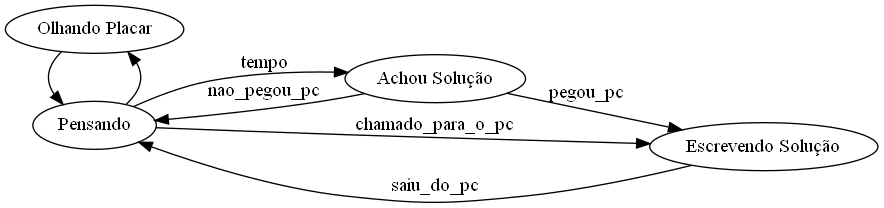
\includegraphics{fsm.png}
    \caption{Caption}
    \label{fig:my_label}
\end{figure}



\section{Conclusão}

% TODO:

\medskip
\printbibliography

\end{document}
